\subsection{Main Effects Models}\label{main-effects-models}

The following models assess the main effects of closed-form cultural
matching, open-ended cultural matching, and network opacity on the odds
of tie persistence. Model 1 shows that closed-form matches independently
predict persistence. Model 2 introduces open-ended matches,
demonstrating the value of incorporating both open and closed-form
items. Model 3 incorporates network opacity (the number of ``Don't
know'' responses regarding an alter's preferences). The main effects
model reveals that a lack of shared cultural knowledge signals a weaker
tie.

\begin{table}

\caption{\label{tbl-models}Odds Ratios for Tie Persistence (Main Effects
Models)}

\centering{

\centering
\begin{talltblr}[         %% tabularray outer open
entry=none,label=none,
note{}={+ p \num{< 0.1}, * p \num{< 0.05}, ** p \num{< 0.01}, *** p \num{< 0.001}},
]                     %% tabularray outer close
{                     %% tabularray inner open
colspec={Q[]Q[]Q[]Q[]},
hline{2}={1-4}{solid, black, 0.05em},
hline{36}={1-4}{solid, black, 0.05em},
hline{1}={1-4}{solid, black, 0.08em},
hline{39}={1-4}{solid, black, 0.08em},
column{2-4}={}{halign=c},
column{1}={}{halign=l},
}                     %% tabularray inner close
& Model 1: Closed & Model 2: + Open & Model 3: + Opacity \\
Closed-Form Matches & \num{1.225}*** & \num{1.174}** &  \\
& (\num{0.060}) & (\num{0.059}) &  \\
Open-Ended Matches &  & \num{1.322}*** & \num{1.310}*** \\
&  & (\num{0.072}) & (\num{0.071}) \\
Network Opacity &  &  & \num{0.748}*** \\
&  &  & (\num{0.042}) \\
Subjective Closeness: Somewhat & \num{0.526}*** & \num{0.574}*** & \num{0.583}*** \\
& (\num{0.073}) & (\num{0.081}) & (\num{0.082}) \\
Subjective Closeness: Close & \num{0.332}*** & \num{0.365}*** & \num{0.419}*** \\
& (\num{0.075}) & (\num{0.083}) & (\num{0.097}) \\
Tie Duration (Years) & \num{1.026} & \num{1.015} & \num{0.987} \\
& (\num{0.048}) & (\num{0.048}) & (\num{0.048}) \\
Tie Duration Squared & \num{0.998} & \num{0.999} & \num{1.000} \\
& (\num{0.003}) & (\num{0.003}) & (\num{0.003}) \\
Ego: Woman & \num{1.084} & \num{1.045} & \num{1.016} \\
& (\num{0.404}) & (\num{0.392}) & (\num{0.385}) \\
Alter: Woman & \num{1.414}* & \num{1.300} & \num{1.247} \\
& (\num{0.240}) & (\num{0.224}) & (\num{0.217}) \\
Ego Woman × Alter Woman & \num{0.622}+ & \num{0.714} & \num{0.750} \\
& (\num{0.163}) & (\num{0.190}) & (\num{0.202}) \\
Roommate/Dormmate & \num{1.117} & \num{1.031} & \num{0.886} \\
& (\num{0.441}) & (\num{0.413}) & (\num{0.357}) \\
Friend & \num{0.811} & \num{0.775} & \num{0.727} \\
& (\num{0.224}) & (\num{0.217}) & (\num{0.204}) \\
Frequency: Weekly/Daily & \num{1.120} & \num{1.158} & \num{1.115} \\
& (\num{0.184}) & (\num{0.192}) & (\num{0.187}) \\
Race Homophily: Same Race & \num{0.967} & \num{0.961} & \num{0.921} \\
& (\num{0.191}) & (\num{0.191}) & (\num{0.185}) \\
Race Homophily: Unknown & \num{0.162}*** & \num{0.165}*** & \num{0.157}*** \\
& (\num{0.030}) & (\num{0.031}) & (\num{0.030}) \\
Time Period: Wave 2-5 & \num{0.053}*** & \num{0.074}*** & \num{0.063}*** \\
& (\num{0.018}) & (\num{0.025}) & (\num{0.022}) \\
Time Period: Wave 5-6 & \num{0.090}*** & \num{0.120}*** & \num{0.088}*** \\
& (\num{0.031}) & (\num{0.042}) & (\num{0.032}) \\
Num.Obs. & \num{3251} & \num{3251} & \num{3251} \\
AIC & \num{2562.3} & \num{2536.7} & \num{2518.5} \\
BIC & \num{2665.8} & \num{2646.3} & \num{2628.1} \\
\end{talltblr}

}

\end{table}%

\subsubsection{Marginal Effects}\label{marginal-effects}

\textbf{Figure Figure~\ref{fig-combined}} visualizes the marginal effect
(calculated as the change from the minimum to the maximum value) of
closed-form matches, open-ended matches, and network opacity on the
predicted probability of tie persistence.

\begin{figure}

\centering{

\pandocbounded{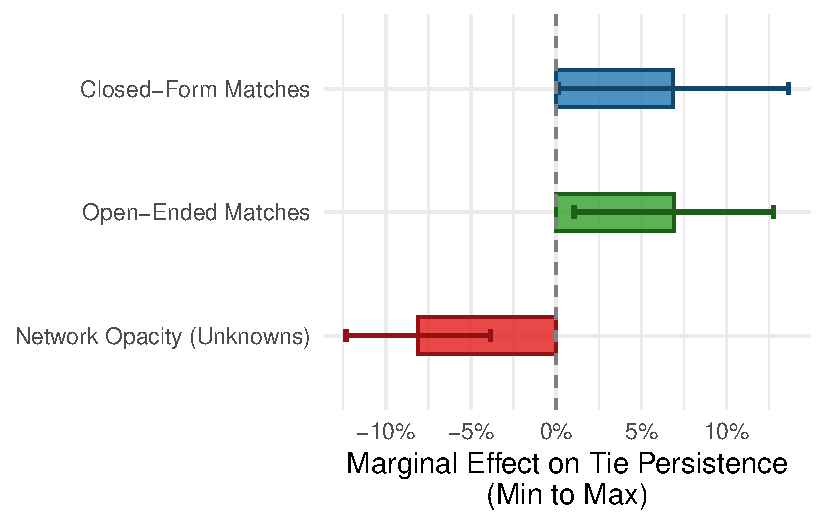
\includegraphics[keepaspectratio]{analysis_files/figure-pdf/fig-combined-1.pdf}}

}

\caption{\label{fig-combined}Marginal Effects of Cultural Matches and
Network Opacity (Min to Max)}

\end{figure}%

\subsection{Subjective Closeness
Interactions}\label{subjective-closeness-interactions}

To test whether the protective effects of cultural matching or the
detrimental effects of network opacity depend on the strength of the
tie, we estimated auxiliary interaction models between subjective
closeness and each of the three cultural variables. While interaction
terms in logistic regression models can be difficult to interpret
directly from coefficients due to the non-linear link function,
computing predicted probabilities across the range of the variables
provides a clearer picture of the underlying dynamics.

\textbf{Figure Figure~\ref{fig-closeness-interactions}} plots the
marginal effects of the three cultural variables across the three levels
of subjective closeness.

\begin{figure}

\centering{

\pandocbounded{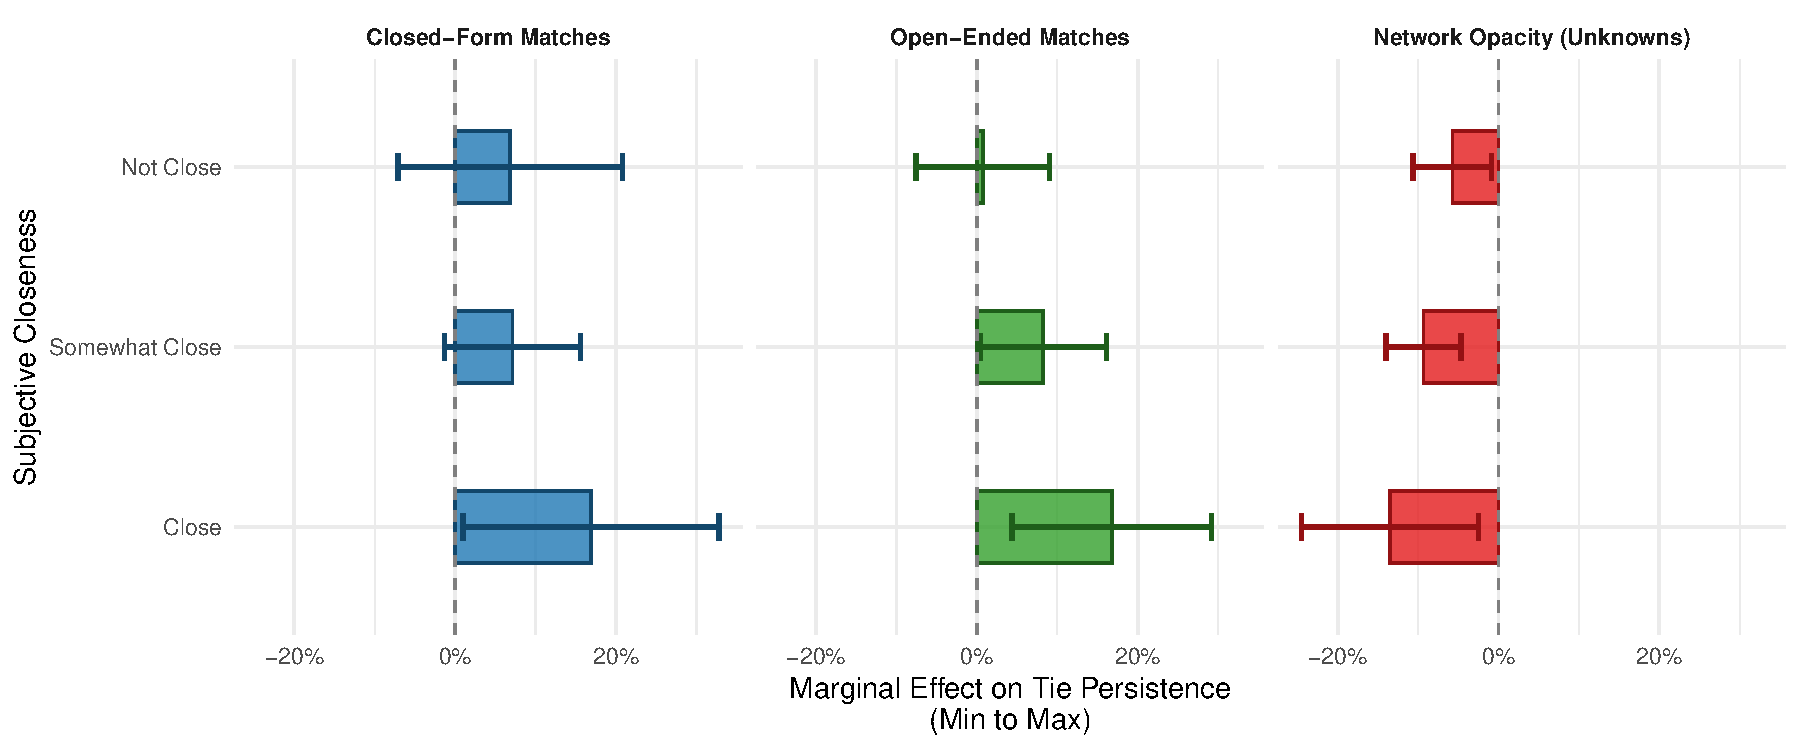
\includegraphics[keepaspectratio]{analysis_files/figure-pdf/fig-closeness-interactions-1.pdf}}

}

\caption{\label{fig-closeness-interactions}Predicted Probability of Tie
Persistence by Cultural Matching, Network Opacity, and Subjective
Closeness}

\end{figure}%

As the marginal effects plot clearly demonstrates, the role of cultural
matching varies substantially by subjective closeness. For ``Not Close''
ties (the steepest slopes), an increase in shared cultural
tastes---whether measured through closed-form domains or open-ended
activities---dramatically increases the probability of tie persistence.
Conversely, for ties that are already ``Close,'' the slope is
essentially flat. This suggests that shared cultural tastes provide
critical scaffolding that helps weak ties survive, whereas strong ties
are resilient to decay regardless of cultural matching. Similarly,
network opacity exerts its most severe negative effect on ties that are
not subjectively close. \#\# Appendix: Descriptive Statistics

{

\begin{longtable}[]{@{}lrrrr@{}}

\caption{\label{tbl-descriptives-cont}Descriptive Statistics for
Continuous Variables}

\tabularnewline

\toprule\noalign{}
Variable & Mean & SD & Min & Max \\
\midrule\noalign{}
\endhead
\bottomrule\noalign{}
\endlastfoot
Closed-Form Matches & 2.12 & 1.47 & 0.00 & 6 \\
Open-Ended Matches & 2.44 & 1.32 & 0.00 & 5 \\
Cultural Network Opacity & 0.81 & 1.51 & 0.00 & 6 \\
Tie Duration (Years) & 3.01 & 4.19 & 0.08 & 20 \\

\end{longtable}

}

{

\begin{longtable}[]{@{}llrr@{}}

\caption{\label{tbl-descriptives-cat}Descriptive Statistics for
Categorical Variables}

\tabularnewline

\toprule\noalign{}
Variable & Category & N & Percent \\
\midrule\noalign{}
\endhead
\bottomrule\noalign{}
\endlastfoot
Alter Gender & Men & 1160 & 53.5 \\
Alter Gender & Women & 1007 & 46.5 \\
Ego Gender & Men & 1127 & 52.7 \\
Ego Gender & Women & 1010 & 47.3 \\
Friend & No & 236 & 10.9 \\
Friend & Yes & 1939 & 89.1 \\
Race Homophily & Heterophilous & 217 & 10.0 \\
Race Homophily & Homophilous & 500 & 23.0 \\
Race Homophily & Unknown & 1458 & 67.0 \\
Roommate/Dormmate & No & 2062 & 94.8 \\
Roommate/Dormmate & Yes & 113 & 5.2 \\
Subjective Closeness & Close & 302 & 14.1 \\
Subjective Closeness & Not Close & 712 & 33.3 \\
Subjective Closeness & Somewhat Close & 1127 & 52.6 \\
Tie Persisted & No & 1489 & 68.5 \\
Tie Persisted & Yes & 686 & 31.5 \\
Time Period & Wave 1 to 2 & 104 & 4.8 \\
Time Period & Wave 2 to 5 & 1365 & 62.8 \\
Time Period & Wave 5 to 6 & 706 & 32.5 \\

\end{longtable}

}




\end{document}
